\documentclass{article}
\usepackage[utf8]{inputenc}
\usepackage{hyperref}
\usepackage{mathtools}
\usepackage{graphicx}
\usepackage{scrextend}

\title{DT057A Project}
\author{raho1501 \& majo1412 \& mafl1400}
\date{May 2019}

\begin{document}

\maketitle

\section{Part I: PRNG and Random Variables} \label{part1}
  \subsection{LCG - Linear Congruential Generator}
    For this project we were tasked to create a LCG\footnote{Linear Congruential Generator}. 
    A LCG uses a recurrence relation to create pseudo random uniformly distributed values, see equation \ref{recrel} for the relation used.
    \begin{equation} \label{recrel}
      X_{n+1} = (aX_{n} + c)\ mod\ m
    \end{equation}
    We then implemented this code in C++ in a file called \href{https://github.com/NoRines/simulerings_projekt/blob/master/lcg.h}{\emph{lcg.h}}.
    Using this LCG we were then tasked to test and compare it against the NS3 UniformRandomVariable generator. 
    We were to generate 1000 different values using provided parameters and then compare the generated values against the NS3 implementation.
    To test our implementation we were provided these paramaters:
    \begin{align*}
      a=13 \\
      m=100 \\
      c=1 \\
      seed=1
    \end{align*}
    When we had ran our implementation of a uniform random number generator we then could 
  \subsection{ITM - Inverse Transform Method}

\begin{enumerate}
  \item A LCG random generator was created in a file named "lcg.h" for generating random uniformed numbers. The file can be found in the git repo.
  \item 1000 values were generated and transformed onto the range [0,1] by calling the function "norm\_gen()" in the "lcg.h" header. A bulk function was also created if the 1000 values were in an array, then the GPU accelerated function "transformKernel(*input, mod, output,1000)" was called, which can be found in the header "func.cuh".
  \item Our function was compared with the ns3 implementation and the result was that our implementation was worse. Ours were cyclic while the ns-3 wasn't as obviously-cyclic.
  \item The ns3 UniformRandomVariable does not seem to repeat and uses more values between 0 and 1. Using our implementation with the values seed=1, a=13, c=1 and m=100 creates a cycle with 20 values before repetition. Both are however uniformally distributed. Using a m that is a large prime would mean that we get as many values as possible between 0 and the large prime this is because p \% n != 0 for any prime p and value n < p. Howerer if a and p are coprime then this also results in a simmilar way to using primes as m. So if we want to make the modulo operation as effective as possible we can choose a m that is a power of 2. Then if we choose an odd value as a, a and m are coprime.
  \item Combined Multiple-Recursive Generator. The normal random variable in ns3 uses the polar form of the Box-Muller method which is a rejection sampeling method that aviods using trigometric functions. \url{https://en.wikipedia.org/wiki/Box\%E2\%80\%93Muller_transform}
  \item Our implementation is faster we get a time of 3.320s for ns3 it takes 3.806s. We tested with 10 million generated values. With 1 billion generated values our takes ~18.468s while ns3 takes ~1m 7.544s
  \item Acording to the lectures we can use inverse cdf to function on the generated uniform random variable to create a random variable following the desired distriobution. For exponential distribution we can use the function:$$ F^{-1}_x(u) = \frac{-1}{\beta} * ln(1-u) \implies x \in \exp{(\lambda)} $$
  \item When comparing our implementation with the ns3 implementation we get quite simmilar distributions. However our implementation seems have a bit less variance than the ns3 version.
\end{enumerate}


\section{Part II: Mathematical Modelling of a system of Queues} \label{part2}
\begin{figure}[h!]
  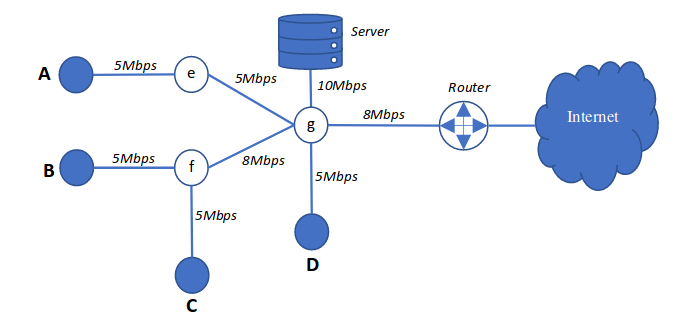
\includegraphics[width=\linewidth]{netmap.png}
  \caption{Network topology}
  \label{fig:netmap}
\end{figure}
By inspecting the figure \ref{fig:netmap} we made a Kleinrock approximation to calculate the average number of packets in the system.
\begin{table}[h]
\centering
\label{Arrivalrates}
\caption{Arrival rates}
\begin{tabular}{|l|l|l|}
\hline
$\lambda_{ij}$ & Calculation & Arrival rate (Packets/s) \\ \hline
$\lambda_{ae}$ & $\frac{1}{2ms}$  & 500 \\ \hline
$\lambda_{bf}$ & $\frac{1}{2ms}$  & 500 \\ \hline
$\lambda_{cf}$ & $\frac{1}{0.5ms}$  & 2000 \\ \hline
$\lambda_{dg}$ & $\frac{1}{1ms}$  & 1000 \\ \hline
$\lambda_{fg}$ & $\lambda_{bf} + \lambda_{cf}$  & 2500  \\ \hline
$\lambda_{eg}$ & $\lambda_{ae}$ & 500 \\ \hline
$\lambda_{gs}$ & $\lambda_{fg} + \lambda_{dg} + \lambda_{eg}$ & 4000 \\ \hline
\end{tabular}
\end{table}
We then calculated the arrivalrate based on the interarrival times and present them in table \ref{Arrivalrates}. We then calculated the service rates which were based on the available bandwidth on the channel between each node. These were then presented in table \ref{departurerates}.
\begin{table}[h]
\centering
\label{departurerates}
\caption{Departure rates}
\begin{tabular}{|l|l|}
\hline
$\mu_{ij}$ & Service rate(Packets/s)\\ \hline
$\mu_{ae}$ & 6250 \\ \hline
$\mu_{eg}$ & 6250 \\ \hline
$\mu_{bf}$ & 6250 \\ \hline
$\mu_{cf}$ & 6250 \\ \hline
$\mu_{dg}$ & 6250 \\ \hline
$\mu_{fg}$ & 10000 \\ \hline
$\mu_{gs}$ & 12500 \\ \hline
\end{tabular}
\end{table}
The values presented in the tables \ref{Arrivalrates} and \ref{departurerates} were then inserted into the formula below to calculate the number of packets on each link:
$$N_{ij} = \frac{\lambda_{ij}}{\mu_{ij} - \lambda_{ij} }$$
With the values this becomes the equation-set 1 below:
$$N_{ae} = \frac{\lambda_{ae}}{\mu_{ae} - \lambda_{ae} } \implies \frac{500}{6250 - 500 } = 0.0869565 $$
$$N_{eg} = \frac{\lambda_{eg}}{\mu_{eg} - \lambda_{eg} } \implies \frac{500}{6250 - 500 } = 0.0869565 $$
$$N_{bf} = \frac{\lambda_{bf}}{\mu_{bf} - \lambda_{bf} } \implies \frac{500}{6250 - 500 } = 0.0869565 $$
$$N_{cf} = \frac{\lambda_{cf}}{\mu_{cf} - \lambda_{cf} } \implies \frac{2000}{6250 - 2000 } = 0.470588 $$
$$N_{dg} = \frac{\lambda_{dg}}{\mu_{dg} - \lambda_{dg} } \implies \frac{1000}{6250 - 1000 } = 0.190476 $$
$$N_{fg} = \frac{\lambda_{fg}}{\mu_{fg} - \lambda_{fg} } \implies \frac{2500}{10000 - 2500 } = 0.333333 $$
$$N_{gs} = \frac{\lambda_{gs}}{\mu_{gs} - \lambda_{gs} } \implies \frac{4000}{12500 - 4000 } = 0.470588 $$
$$Equations\ 1.\ Individual\ number\ of\ packets.$$

Later we used the formula below to calculate the average number of packets in the whole system:
$$ \overline{N} = \sum N_{ij} $$
Which gave us the resulting equation-chain:
$$ \overline{N} = \sum N_{ij} = \frac{500}{6250 - 500 } + \frac{500}{6250 - 500 } + \frac{500}{6250 - 500 } + \frac{2000}{6250 - 2000 } + $$ 
$$ \frac{1000}{6250 - 1000 } + \frac{2500}{10000 - 2500 } + \frac{4000}{12500 - 4000 } = 1.638898 packets $$ 


Which concludes the section with the answers to the questions on part 2. The average number of packets are 1.638898 packets and the number of packets per link can be found in equations 1.


\section{Part III: Simulations and Results Comparison} \label{part3}

\begin{itemize}
    \item Run the simulation and measure:
    \begin{itemize}
        \item The average number of request packets queued at the link between and the Router (g $\rightarrow$ Server)
        \begin{addmargin}[1em]{2em}
        As can be seen in the calculations from section \ref{part2} the average number of packets between node g and the server was about ~0.47 packets.
        When simulated the results acquired were very different.
        The average number of packets between node g and the server was about ~0.064 packets which is significantly smaller than the calculated results.
        We have two theories for the reason for this difference.
        \textbf{First} the calculations use the Kleinrock independence approximation which may not be a good approximation for the system.
        This is because the system has quite low traffic while the Kleinrock approximation works better for high traffic systems.
        We tested halving all the data rates in the system and got results more close to the calculated values.
        \textbf{Second} the simulation might not take into account the packets that are in service by only counting the packets that are in queue.
        This might be responsible for part of the error since the Kleinrock approximation calculates the total number of packets in the point to point connection.
        When measuring the average queue size between g and the router the results are 0.
        This is probably because the router is able to consume the packet fast enough so that no queue has time to form.
        \end{addmargin}
        
        \item The average queuing delay and the total average delay for the request packets traversing the link f $\rightarrow$ g
        \begin{addmargin}[1em]{2em}
        By creating a flow monitor statistical analyser file we calculated the average total delay for f $\rightarrow$ g.
        By taking the delay sum for the flow by checking the total delay values in the statistical analyser file.
        $$\frac{((b \rightarrow g) - (b \rightarrow f)) + ((c \rightarrow g) - (c \rightarrow f))}{number\ of\ packets}$$
        The delay was calculated to be about ~0.123 milliseconds.
        
        \end{addmargin}
    \end{itemize}
    
    \item Compare the results you get from the simulation with the one you obtained in Part II.
    \begin{addmargin}[1em]{2em}
    I think we did this already.
    \end{addmargin}
    
    \item Measure the delay between A and the Server and between the Server and A.
    \begin{addmargin}[1em]{2em}
    A to server: 0.454 milliseconds.
    Server to A: 0.478 milliseconds.
    \end{addmargin}
    
    \item Replace each P2P link with a bus using CSMA/CD do not change the data rate or delay.
    \begin{addmargin}[1em]{2em}
    When replacing all the point to point connections with CSMA busses with collision detection a very large queue is built from the server to g. This is most likely due to the larger flow of packets going into g from node F, E and D and only one point out to the server. So when the responses from the server is on its way back, they have to share the bus with the input from the three nodes. Because of this there is a huge backlog at node g. 
    \end{addmargin}
    
    \item Run the simulation but this time use the custom PRNG that you implemented in Part I to generate the exponential packet size and the exponential time between packets. Which differences do you observe?
    \begin{addmargin}[1em]{2em}
    When we changed to our implementation of the PRNG we got similar result as before but with slightly smaller values. The average queue size in G dropped to about 0.055 on G to server, to 0 on G to router (which is unchanged) and 0.150 on F to G. The delay from F to G was unchanged, the delay from server to A was 0.46ms which is slightly lower than before, and from A to server was 0.48 ms which is slightly more than previously. These are inside the error bounds so they can be deemed unchanged. 
    
    However the overall difference when we change to our PRNG implementation was negligible and the only thing we noticed was a more predictable pattern in the packet sizes.
    \end{addmargin}
\end{itemize}

\subsection{Implementation}
We decided to use the ns3 discrete event network simulator.


\subsubsection{Network topology}

\subsubsection{Scheduling}

\subsubsection{Logging method}

\subsection{Simulation}

\subsubsection{Evaluation}

\subsubsection{Comparisons}

\section{Conclusions}

\end{document}

\end{document}